在本次实验中,我们在L= 50.0cm,n=1,ρ[2\#]=0.00098kg/m条件下,探究弦振动频率与T的关系。
\begin{table}[h]
    \centering
    \begin{tabular}{|c|c|}
        \hline
        T(N)  & f(Hz)  \\
        \hline
        1.96  & 43.35  \\
        3.92  & 61.43  \\
        5.88  & 75.71  \\
        7.84  & 88.08  \\
        9.80  & 98.13  \\
        11.76 & 107.26 \\
        \hline
    \end{tabular}
    \caption{弦振动频率与T的关系实验的测量数据}
    \label{6283f961}
\end{table}

n=1时,$\Delta_A$无法计算,而$\Delta_B$=0.01,因此取$\Delta$=0.01。

由\ref{6283f961}这样的数据,我们利用Python程序,可以得到\ref{e75eff9d}。
\begin{figure}[h]
    \centering
    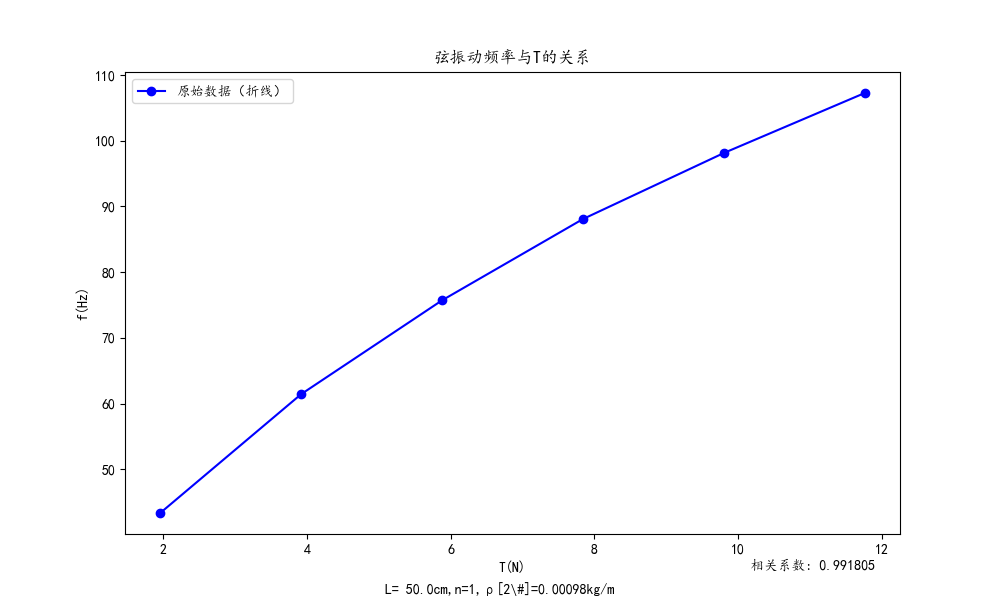
\includegraphics[scale=0.5]{2_original.png}
    \caption{弦振动频率与T的关系的原始数据}
    \label{e75eff9d}
\end{figure}

很容易发现此时并非线性关系,我们选取合适的回归方式进行拟合。

取ln后,我们可以得到拟合结果如下图所示。
\begin{table}[h]
    \centering
    \begin{tabular}{|c|c|}
        \hline
        ln[T(N)] & ln[f(Hz)] \\
        \hline
        0.67     & 3.77      \\
        1.37     & 4.12      \\
        1.77     & 4.33      \\
        2.06     & 4.48      \\
        2.28     & 4.59      \\
        2.46     & 4.68      \\
        \hline
    \end{tabular}
    \caption{弦振动频率与T的关系实验的拟合数据}
    \label{2f68f884}
\end{table}
\begin{figure}[h]
    \centering
    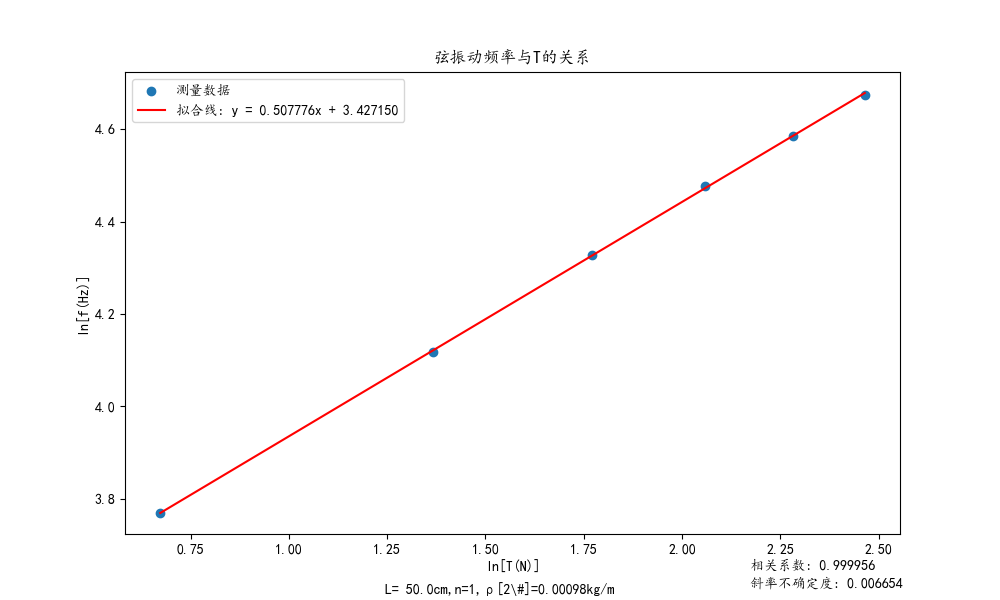
\includegraphics[scale=0.5]{2.png}
    \caption{弦振动频率与T的关系的拟合结果}
    \label{ac188e73}
\end{figure}


由图可知,拟合结果为\ref{ac188e73}:$y=0.507776x+3.427150$。
\textbf{相关系数}为: 0.999956。
根据斜率不确定度的计算公式:
\begin{align}
    \Delta_{slope} & =t(N-2)\cdot S_{slope} \\ & = t(N-2)\cdot slope\cdot  \sqrt{\frac{\frac{1}{r^2}-1}{N-2}}\\ & = t(4)\cdot 0.5077755628990771\cdot \sqrt{\frac{\frac{1}{0.9999555698343207^2-1}}{6-2}} \\ &= 0.006654
\end{align}